\chapter{Additional Design Details}
\label{app:extras}

This appendix gives the parts of the design that Chapter~\ref{chap:design} summarises or only
refers to: moderation, plans and automatic captions (Section~\ref{sec:extras-design}), and the
verification of an account, the permissions of the staff roles and the collections of moderation
(Sections~\ref{sec:security-design} and~\ref{sec:database-design}).

\section{Content Moderation Design}
\label{sec:moderation-design}

Moderation combines automatic screening, which acts on every video before it is published, with
human decisions that correct it and are recorded so that its errors can be measured.
Figure~\ref{fig:moderation-sequence} shows the whole flow.

\begin{figure}[htbp]
\centering
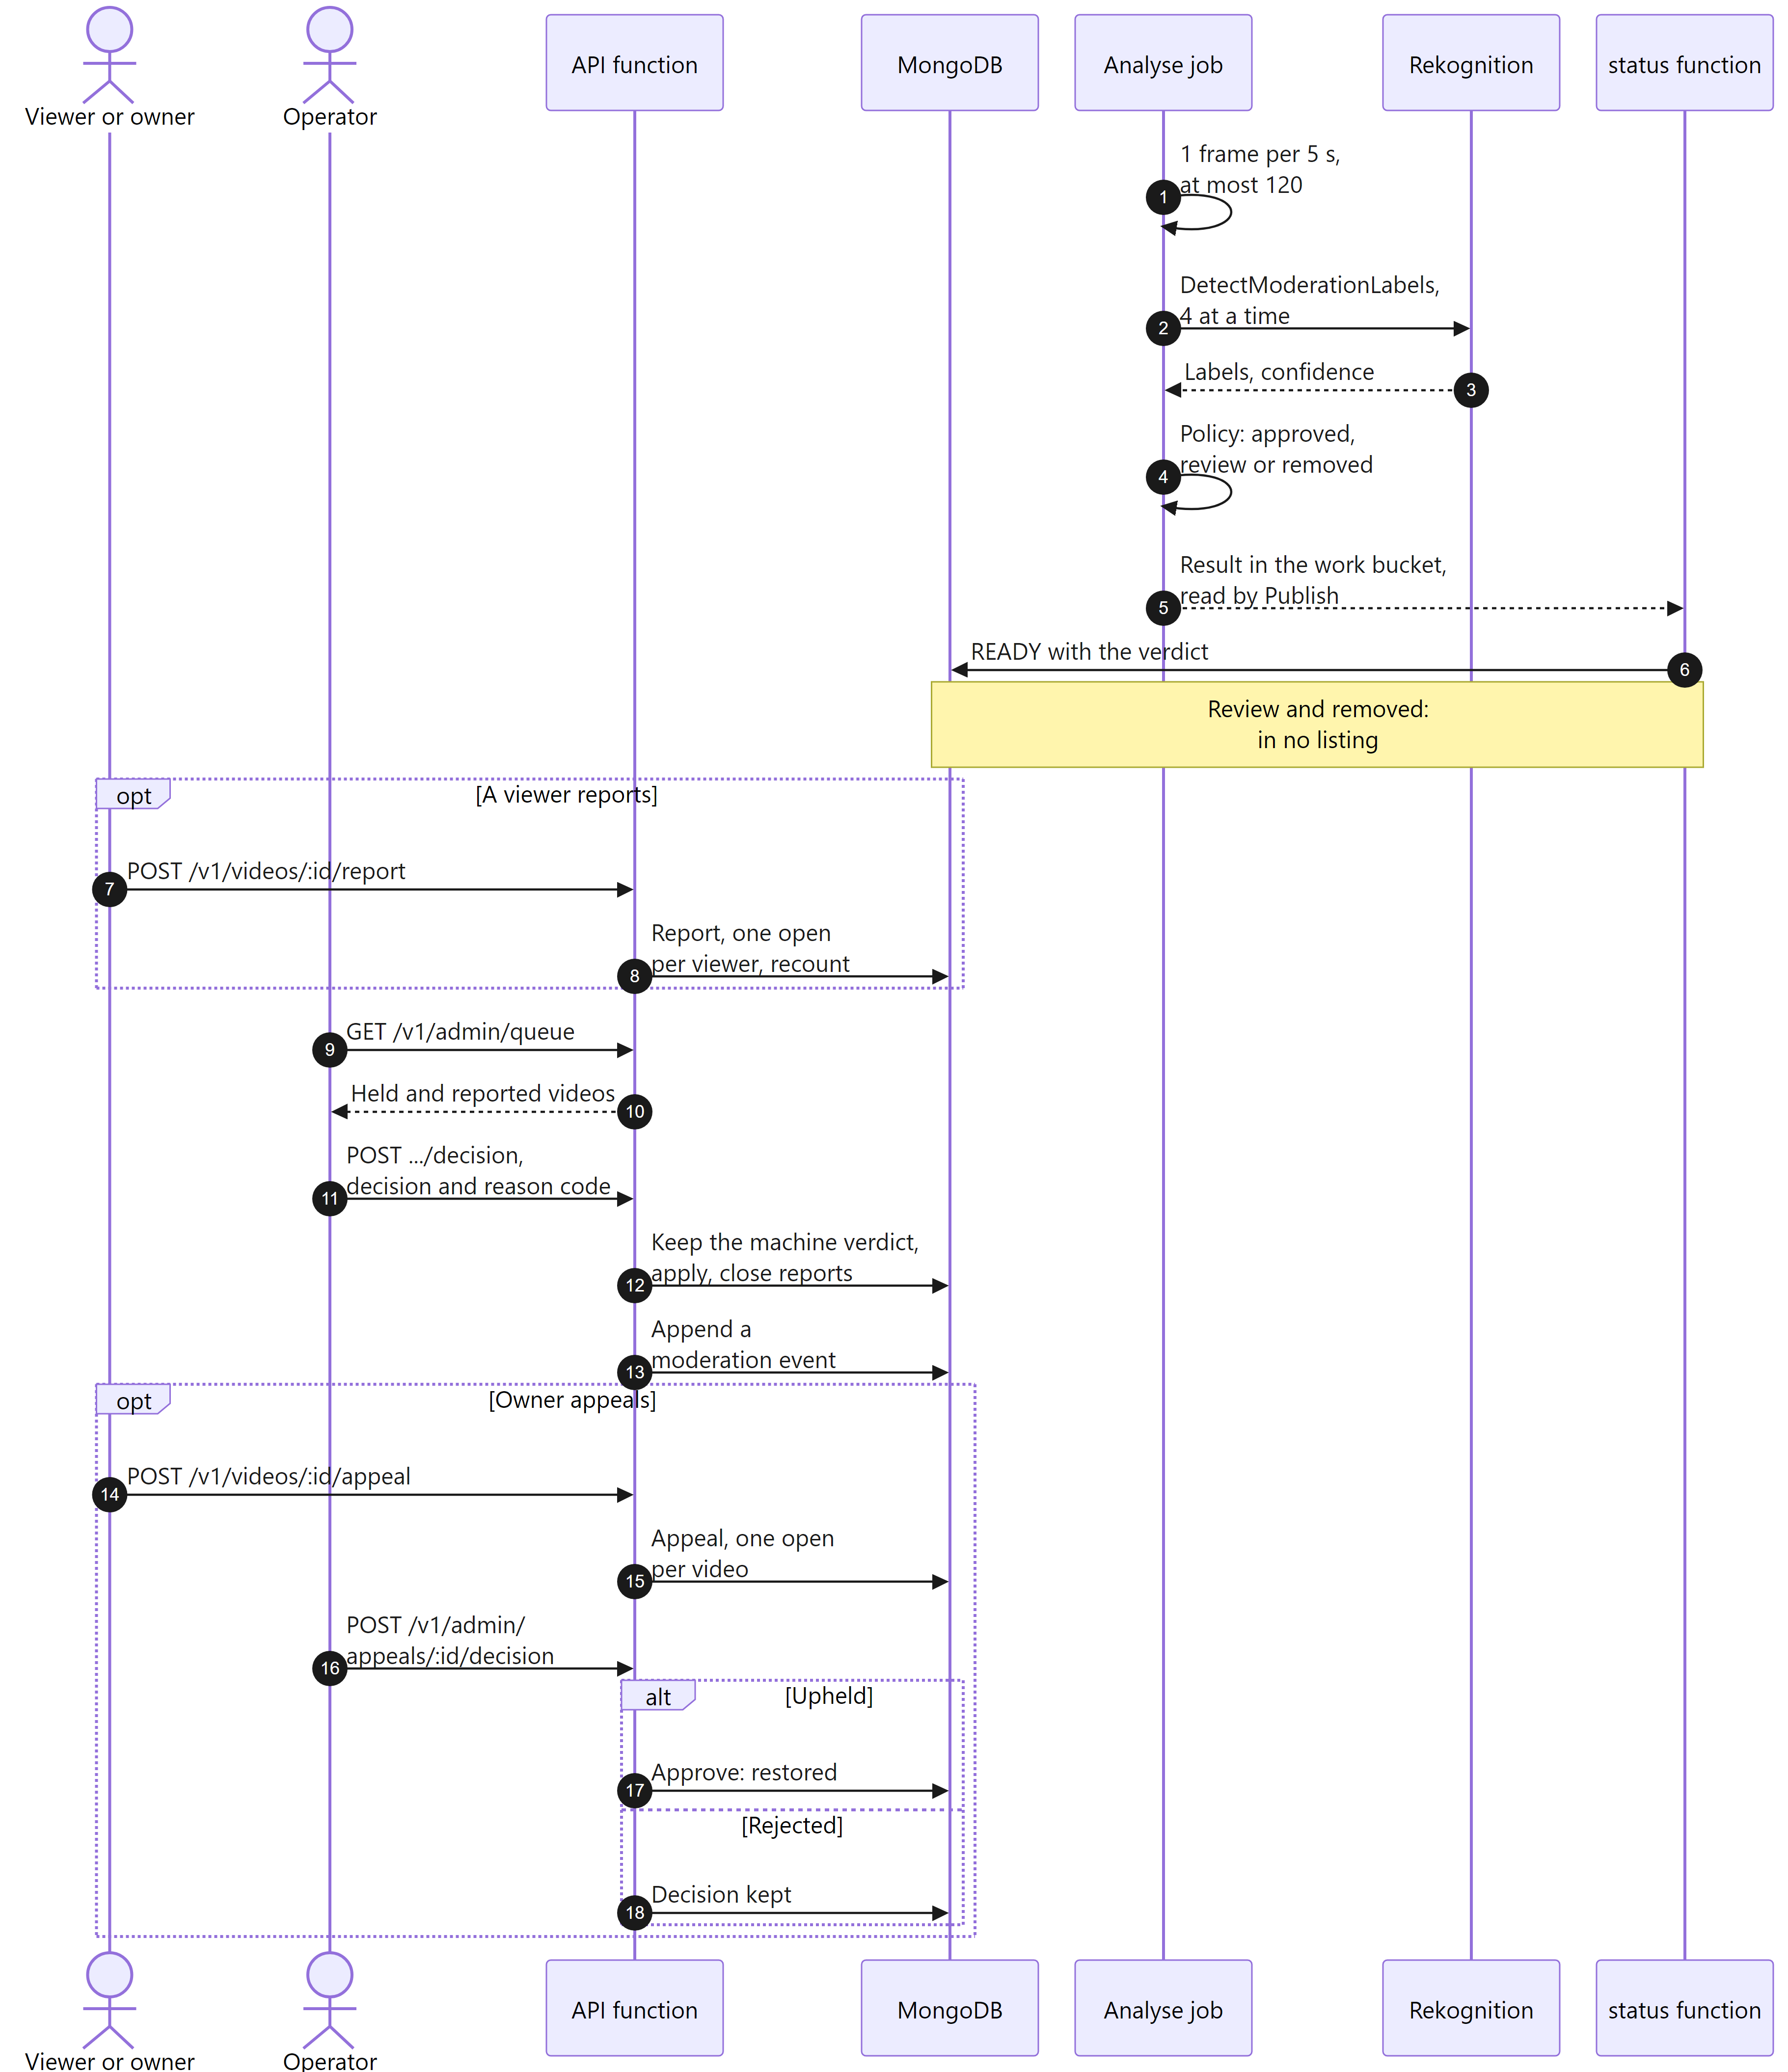
\includegraphics[width=0.95\textwidth]{images/19-moderation-sequence.png}
\caption{\textit{Moderation: automatic screening, a viewer's report, an operator's decision and the
owner's appeal}}
\label{fig:moderation-sequence}
\end{figure}

\subsection{Automatic Screening}
\label{sec:screening-design}

The \name{analyse} job takes one frame every five seconds, at most 120 frames, so the interval
widens for long videos and the cost of a video is bounded. Each frame goes to Amazon Rekognition,
four at a time, and the labels are mapped by a shared policy to block, review or ignore, following the
label taxonomy of the service~\cite{awsrekognitionmoderation}. Labels below 60\% confidence are
treated as noise. A block label at 90\% confidence or more removes the video; any other relevant
label holds it for review. A throttled call to Rekognition is retried by the client with adaptive
back-off, up to five attempts, so a burst of uploads slows the screening rather than skipping frames. Labels such as graphic violence
in animation or illustration are lowered to review, since fiction is not the same as a recording. A
video with violence that may stay is published behind a warning that the viewer dismisses. Screening
fails closed: when no frame, or less than 80\% of the planned frames, could be analysed, the video is
held for review rather than published. Avatars, banners and custom thumbnails pass through the same
policy and are refused on any relevant label.

Screening is billed per frame, so an administrator can switch it for new videos in the staff
console, as for automatic captions (Section~\ref{sec:captions-design}). The switch lives in the
database, and the processing containers hold no database credentials, so they never read it:
\name{MarkProcessing} reads it when the workflow starts and the state machine passes it to the
\name{analyse} job as an environment value that overrides the one of the job definition. A change
therefore applies to the videos that start processing after it, and without a stored value the
default set by Terraform applies. A video processed with screening off is published as approved
with the source \name{disabled}, so it never enters the error rates of
Section~\ref{sec:review-design}; viewers can still report it and operators still decide on it.

\subsection{Review, Appeals and Audit}
\label{sec:review-design}

An operator decides on every held or reported video with a decision, approve or remove, and a reason
code from a closed list for that decision, such as a model error, fiction, a confirmed violation or a
report upheld. Before the first human decision overrides it, the verdict of the machine is kept, and
each decision is appended to the event log with an outcome class that compares the two, as
Table~\ref{tab:outcome-classes} shows. An operator cannot change a decision taken by an
administrator. The owner of a removed or held video can appeal while no other appeal on it is open,
and an upheld appeal approves the video with the reason ``appeal upheld''.

\begin{table}[H]
\centering
\caption{Outcome classes of a human decision against the machine verdict}
\label{tab:outcome-classes}
\small
\begin{tabular}{l l l}
\toprule
\textbf{MACHINE VERDICT} & \textbf{HUMAN DECISION} & \textbf{OUTCOME} \\
\midrule
removed & approve & false positive \\
review & approve & flag noise \\
approved & approve & true negative \\
approved & remove & false negative \\
review or removed & remove & true positive \\
none recorded & either & unclassified \\
\bottomrule
\end{tabular}
\end{table}

Decisions alone cannot measure what the screening misses, because nobody reviews a video that the
machine approved and no viewer reported. The random audit fills this gap: an administrator draws a
sample of videos that the machine alone approved, an operator labels each one pass or fail, and a
failed video is removed. From these records the console computes three rates, each with a 95\%
Wilson interval, which stays meaningful for small samples and rates near zero, and the sample size
beside it. The first is the share of reviewed automatic removals that a person reversed. Its
denominator is the removals, not every acceptable video, so it estimates the false discovery rate of
removals (one minus their precision) rather than the false positive rate. The second is the
precision of holds. The third is the share of audited approvals that failed, which estimates the
false omission rate of approvals rather than the false negative rate, since its denominator is the
approved videos and not every violating one. Removals reach a person when an operator opens them or
the owner appeals, not at random, so the first rate can be biased toward contested cases; only the
third comes from a random sample.

\subsection{Roles and Separation of Duties}
\label{sec:roles-design}

The roles are kept apart so that no person checks their own work. Operators decide and label;
auditors read the rates and the log but hold no permission that changes anything; administrators
manage roles and draw samples, and can act as either. The last administrator cannot be demoted, and
every change of role is logged with who made it.

\section{Plans, Payment and Automatic Captions}
\label{sec:plans-design}

Some parts of the system cost money per use: storage and encoding grow with the size and length of
a video, and speech recognition is billed per second of audio. The platform plans decide how far each
creator may use these parts, and they pay for the generous ones.

\subsection{Plans and Entitlements}
\label{sec:entitlements}

Table~\ref{tab:plans} lists the four plans. Their limits are defined in one shared module, and every
other part of the code asks a single function for the entitlements of a user at a given moment
instead of testing a plan name, so the API, the workflow and the caption function cannot disagree
about a limit. Accounts created before the plans existed, on 13~November~2026, keep the limits of Pro
on the free plan, so that nobody lost a right they already had; the processing priority is new and
is not part of what they keep.

\begin{table}[H]
\centering
\caption{Platform plans and their limits}
\label{tab:plans}
\small
\begin{tabularx}{\textwidth}{>{\raggedright\arraybackslash}X r r r r}
\toprule
\textbf{LIMIT} & \textbf{FREE} & \textbf{PLUS} & \textbf{PRO} & \textbf{MAX} \\
\midrule
Price per month, VND & 0 & 49\,000 & 99\,000 & 199\,000 \\
Largest upload & 2~GiB & 5~GiB & 20~GiB & 20~GiB \\
Longest video & 60~min & 180~min & 360~min & 720~min \\
Membership tiers of the channel & 2 & 3 & 5 & 10 \\
Analytics window & 28~days & 90~days & 365~days & 365~days \\
Automatic captions per month & -- & 20~min & 40~min & 80~min \\
Longest video with automatic captions & -- & 15~min & 30~min & 60~min \\
Priority queues & no & yes & yes & yes \\
\bottomrule
\end{tabularx}
\end{table}

Each limit is enforced where the work starts. The upload route refuses a file larger than the plan
allows before it creates anything; the studio refuses a tier beyond the plan and shortens an
analytics window to the longest the plan allows; the workflow reads the plan when it starts, which decides the queues and the longest duration
of Section~\ref{sec:state-machine}; and the caption function reads it before it spends anything. The
length is checked after the probe rather than at upload because only the probe reads the real
duration of the file, and it is cheap: a video over the limit costs three short function calls and
no container.

\subsection{Payment with Stripe}
\label{sec:payment-design}

The platform does not handle card data. A user who chooses a paid plan asks the API for a Stripe
Checkout session in subscription mode with a monthly price in VND, a currency without minor units,
and the reference of the user; the browser is sent to the page that Stripe hosts, and Stripe returns
it to the settings page after the payment~\cite{stripecheckout}. Changes and cancellations happen on
the customer portal that Stripe also hosts.

The browser's return proves nothing, so the plan is set only by the webhook. Stripe sends signed
events for a completed checkout, a created, updated or deleted subscription and a failed payment.
The API checks the signature, inserts the identifier of the event into \name{billingEvents}, whose
unique key makes a redelivered event a no-op, and applies the event to the \name{billing} field of the
user. Every event carries its creation time, and an event older than the last one applied is ignored,
because Stripe does not promise to deliver events in order~\cite{stripewebhooks}. If applying an
event fails, its identifier is removed again so that the retry of Stripe is not taken for a
duplicate. A paid plan counts while Stripe reports the subscription as active, and after a
cancellation or a failed renewal it lasts until the end of the period already paid.

Payments run in the test mode of Stripe, with test cards and no real money, until real payments are
allowed; the code is the same in both modes, and only the key and the signing secret change.

\subsection{Automatic Captions}
\label{sec:captions-design}

Automatic captions are kept outside the transcoding state machine, so that a problem with speech
recognition can never fail a video. The \name{captions} function listens to two events. When a video
is published, it checks the plan of the owner, the duration of the video against the longest video
the plan captions, and the minutes left this month; it then starts one Amazon Transcribe job on the
source, which identifies the language among Vietnamese and English and writes a WebVTT
file~\cite{awstranscribe}. When Transcribe reports that the job has finished, the function copies the
file next to the video as a caption track marked \name{auto}, which the player offers like any other
track; a caption that the owner uploads in the same language replaces it. The job name is derived
from the environment, the video and its upload version, so a redelivered event cannot start a second
job.

The monthly minutes are a budget that two simultaneous videos must not overrun together. The
function reserves the minutes before it starts the job with a single conditional update of the
document of the user and month in \name{captionUsage}: the update adds the seconds of the video only
if the total stays within the plan, so the database itself decides which of two racing reservations
succeeds. A job that fails gives its seconds back. The reservation counts at least fifteen seconds
per video, the minimum that Transcribe bills. Videos without sound, sources over the 2~GB that
Transcribe accepts, and videos that the owner has already captioned are skipped before anything is
reserved, so they cost nothing. Before any of these checks the function reads the switch that an
administrator sets in the staff console; when it is off, no job starts and nothing is reserved.

\section{Accounts, Roles and Moderation Data}
\label{sec:extras-accounts}

Figure~\ref{fig:verification-sequence} shows how the owner of an account is verified, and
Table~\ref{tab:permissions} lists the permissions of each staff role.

\begin{figure}[htbp]
\centering
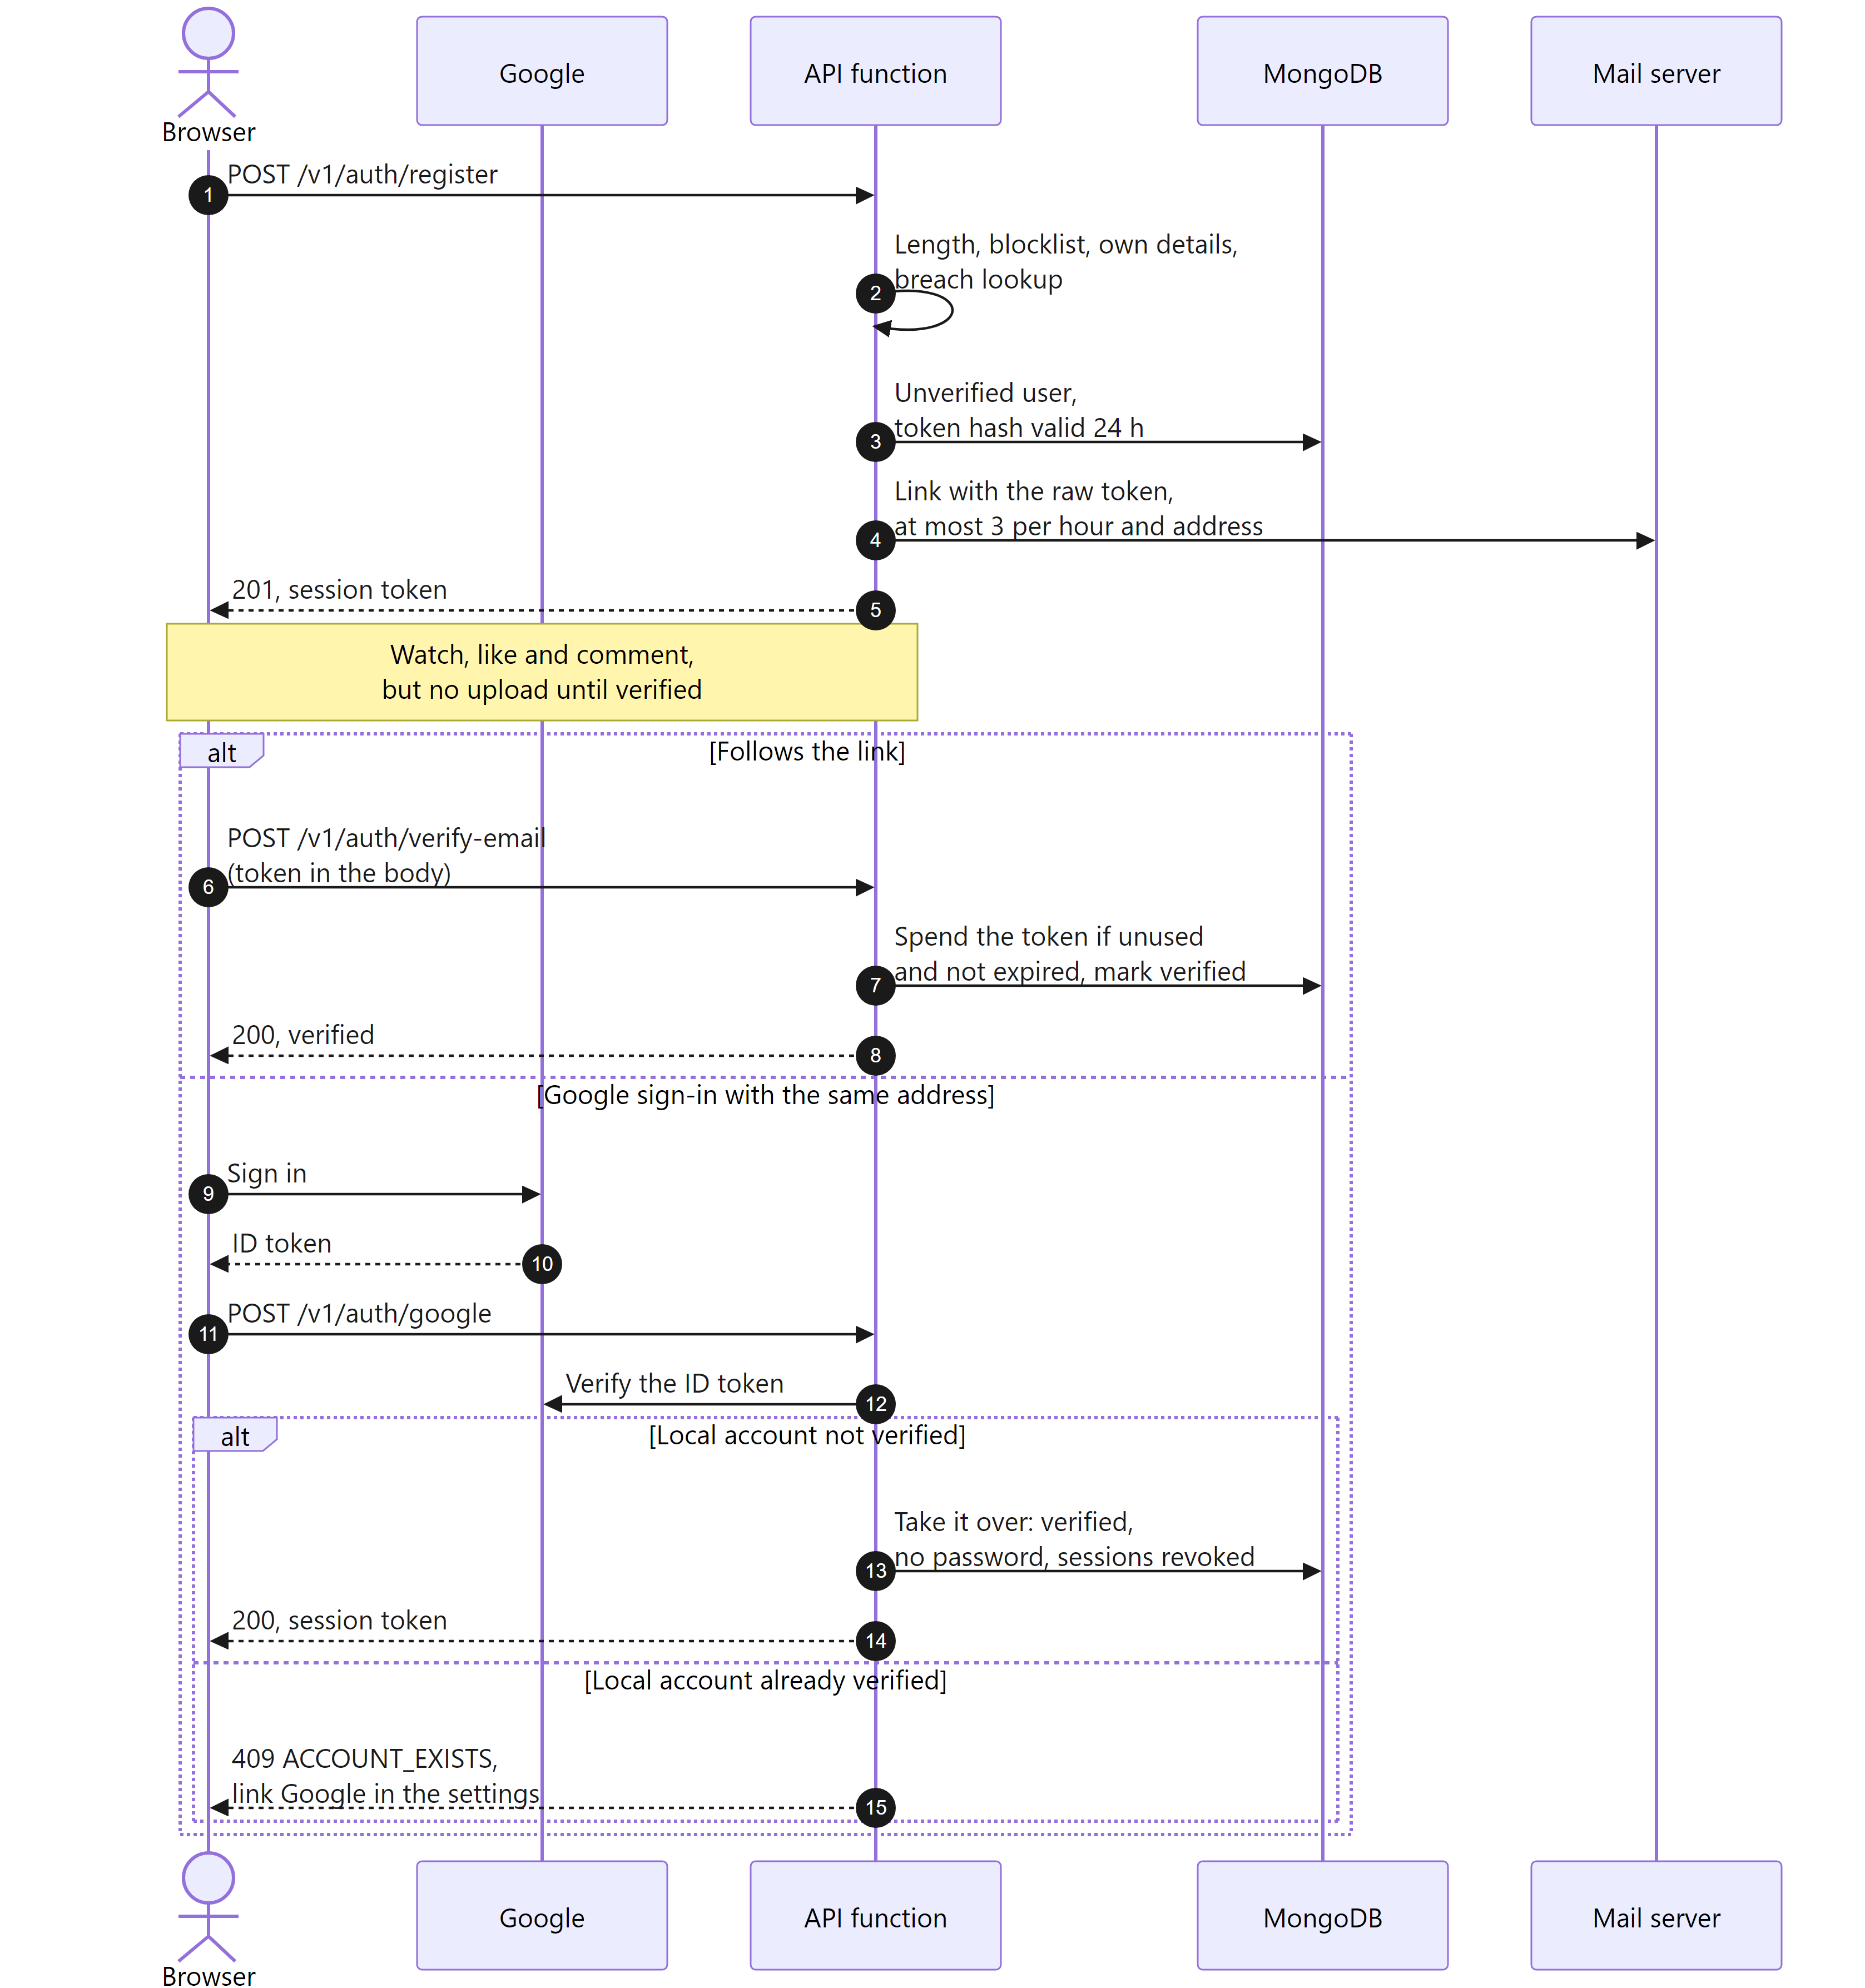
\includegraphics[width=0.92\textwidth]{images/18-verification-sequence.png}
\caption{\textit{Verifying the owner of an account: by the e-mailed link, or by Google sign-in with
the same address}}
\label{fig:verification-sequence}
\end{figure}

\begin{table}[H]
\centering
\caption{Permissions of the staff roles}
\label{tab:permissions}
\small
\begin{tabularx}{\textwidth}{>{\raggedright\arraybackslash}p{0.26\textwidth} >{\raggedright\arraybackslash}X >{\raggedright\arraybackslash}p{0.25\textwidth}}
\toprule
\textbf{PERMISSION} & \textbf{ALLOWS} & \textbf{ROLES} \\
\midrule
moderation:review & Review queue, decisions, reported comments & administrator, operator \\
moderation:appeals & Resolve appeals & administrator, operator \\
moderation:audit & Label audit samples & administrator, operator \\
moderation:sample & Draw audit samples & administrator \\
metrics:read, events:read & Error rates, decision log, role changes & administrator, auditor \\
users:manage & Users and roles & administrator \\
content:viewRemoved & Open removed and held videos & administrator, operator \\
system:read & Overview of users, plans, content and views & administrator \\
settings:manage & Switch screening and automatic captions & administrator \\
\bottomrule
\end{tabularx}
\end{table}

Figure~\ref{fig:moderation-erd} shows the eight collections of moderation and operation. Three of
them are append-only logs, the moderation events, the role changes and the changes of the runtime
switches: the API inserts into them and never updates them, which is what lets an auditor trust
them. The switches themselves are one document, \name{settings/system}.

% Xoay ngang: đặt vừa bề rộng vùng chữ thì chữ dưới 6,2pt khi in.
\begin{sidewaysfigure}
\centering
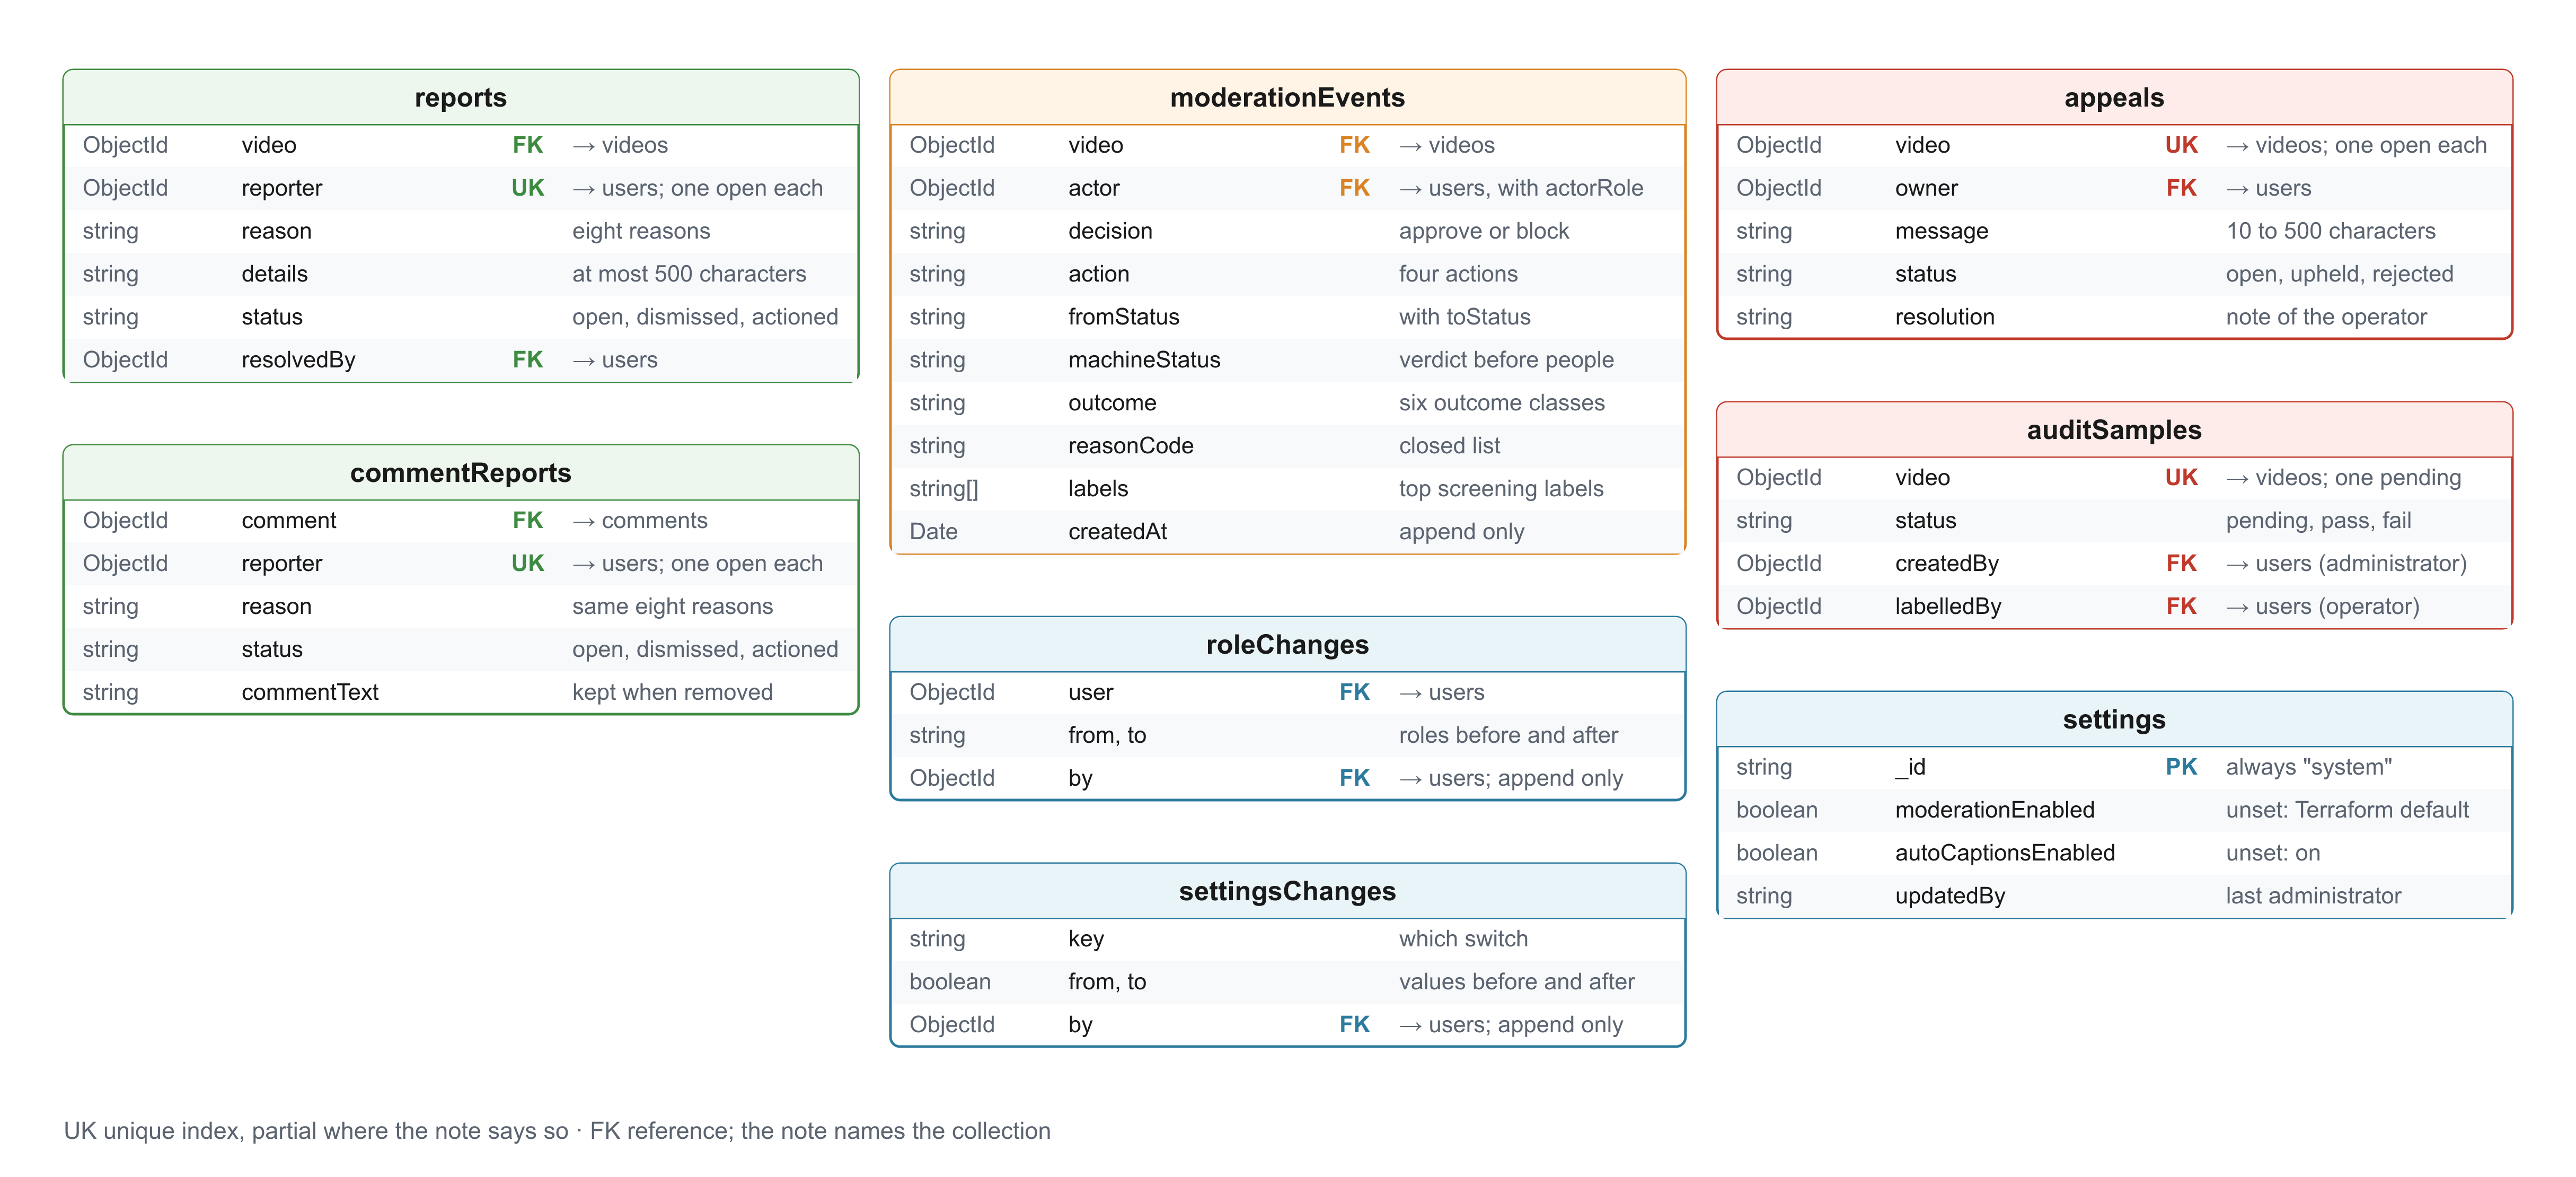
\includegraphics[width=\textheight]{images/09-moderation-erd.png}
\caption{\textit{Collections of moderation and operation}}
\label{fig:moderation-erd}
\end{sidewaysfigure}
